\section{Procedure Interface}

Procedure calls in XMP are almost the same as those in the base language.
%
Procedure calls between other languages or to external libraries
are also allowed if the base language supports them. 

In the below example, a function/subroutine \|sub1()| calls another
function/subroutine \|sub2()| with a {\darray} \|x| as an
argument.

\begin{XCexample}
void sub1(){
#pragma xmp nodes p[2]
#pragma xmp template t[10]
#pragma xmp distribute t[block] onto p
  double x[10];
#pragma xmp align x[i] with t[i]
  sub2(x);
}

void sub2(double a[10]){
#pragma xmp nodes p[2]
#pragma xmp template t[10]
#pragma xmp distribute t[block] onto p
  double a[10];
#pragma xmp align a[i] with t[i]
  :
}
\end{XCexample}

\begin{XFexample}
subroutine sub1()
!$xmp nodes p(2)
!$xmp template t(10)
!$xmp distribute t(block) onto p
  real x(10)
!$xmp align x(i) with t(i)
  call sub2(x)
end subroutine

subroutine sub2(a)
!$xmp nodes p(2)
!$xmp template t(10)
!$xmp distribute t(block) onto p
  real a(10)
!$xmp align a(i) with t(i)
  :
end subroutine
\end{XFexample}

% If the programmer wants to use distributed arrays in arguments as distributed arrays
% in the called procedure,
% %
% you need to redefine the shape of the distributed array in the procedure.

To handle a parameter or dummy argument as a {\bf global data} in the
callee procedure, the programmer need to explicitly distribute it with
an \|align| directive.

\begin{figure}
  \centering
  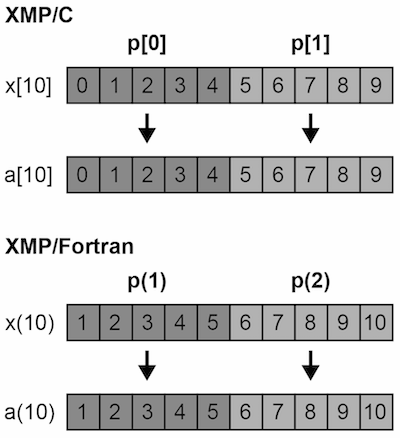
\includegraphics[width=0.9\columnwidth]{figs/destributed_array.png}
  \caption{Passing a global argument to a global parameter.}
\end{figure}

% However, if the programmer wants to use the distributed array in the argument as a
% replicated array in the called procedure, you do not need to redefine
% them.

If no \|align| directive is specified in the callee procedure for a
parameter or dummy argument that is declared as a {\bf global data} in the
caller procedure, it is handled as if it were declared in the callee
procedure as a {\bf local data} on each {\node}, as follows.

\begin{XCexample}
void sub1(){
#pragma xmp nodes p[2]
#pragma xmp template t[10]
#pragma xmp distribute t[block] onto p
  double x[10];
#pragma xmp align x[i] with t[i]
  sub2(x);
}

void sub2(double a[5]){
  :
}
\end{XCexample}

\begin{XFexample}
subroutine sub1()
!$xmp nodes p(2)
!$xmp template t(10)
!$xmp distribute t(block) onto p
  real x(10)
!$xmp align x(i) with t(i)
  call sub2(x)
end subroutine

subroutine sub2(a)
  real a(5)
  :
end subroutine
\end{XFexample}

\begin{figure}
  \centering
  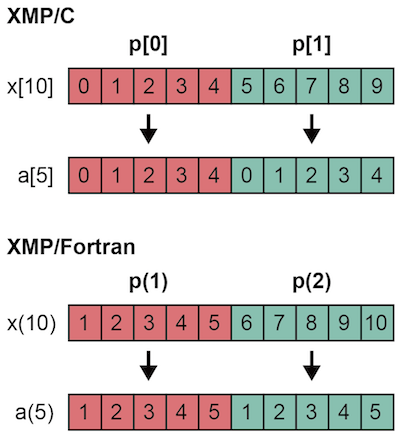
\includegraphics[width=0.9\columnwidth]{figs/duplicated_array.png}
  \caption{Passing a global argument to a local parameter.}
\end{figure}